\pdfminorversion=4
\documentclass[aspectratio=169]{beamer}

\mode<presentation>
{
  \usetheme{default}
  \usecolortheme{default}
  \usefonttheme{default}
  \setbeamertemplate{navigation symbols}{}
  \setbeamertemplate{caption}[numbered]
  \setbeamertemplate{footline}[frame number]  % or "page number"
  \setbeamercolor{frametitle}{fg=white}
  \setbeamercolor{footline}{fg=black}
} 

\usepackage[english]{babel}
\usepackage[utf8x]{inputenc}
\usepackage{tikz}
\usepackage{courier}
\usepackage{array}
\usepackage{bold-extra}
\usepackage{minted}
\usepackage[thicklines]{cancel}
\usepackage{fancyvrb}

\xdefinecolor{dianablue}{rgb}{0.18,0.24,0.31}
\xdefinecolor{darkblue}{rgb}{0.1,0.1,0.7}
\xdefinecolor{darkgreen}{rgb}{0,0.5,0}
\xdefinecolor{darkgrey}{rgb}{0.35,0.35,0.35}
\xdefinecolor{darkorange}{rgb}{0.8,0.5,0}
\xdefinecolor{darkred}{rgb}{0.7,0,0}
\definecolor{darkgreen}{rgb}{0,0.6,0}
\definecolor{mauve}{rgb}{0.58,0,0.82}

\title[2011-11-30-acat-python-cpp]{Lessons learned in Python-C++ integration}
\author{Jim Pivarski}
\institute{Princeton University -- IRIS-HEP}
\date{November 30, 2021}

\usetikzlibrary{shapes.callouts}

\begin{document}

\logo{\pgfputat{\pgfxy(0.11, 7.4)}{\pgfbox[right,base]{\tikz{\filldraw[fill=dianablue, draw=none] (0 cm, 0 cm) rectangle (50 cm, 1 cm);}\mbox{\hspace{-8 cm}\includegraphics[height=1 cm]{princeton-logo-long.png}\hspace{0.1 cm}\raisebox{0.1 cm}{\includegraphics[height=0.8 cm]{iris-hep-logo-long.png}}\hspace{0.1 cm}}}}}

\begin{frame}
  \titlepage
\end{frame}

\logo{\pgfputat{\pgfxy(0.11, 7.4)}{\pgfbox[right,base]{\tikz{\filldraw[fill=dianablue, draw=none] (0 cm, 0 cm) rectangle (50 cm, 1 cm);}\mbox{\hspace{-8 cm}\includegraphics[height=1 cm]{princeton-logo.png}\hspace{0.1 cm}\raisebox{0.1 cm}{\includegraphics[height=0.8 cm]{iris-hep-logo.png}}\hspace{0.1 cm}}}}}

% Uncomment these lines for an automatically generated outline.
%\begin{frame}{Outline}
%  \tableofcontents
%\end{frame}

% START START START START START START START START START START START START START

\begin{frame}{\mbox{ }}
\Large

\vspace{0.5 cm}
This talk is about lessons learned in Python-C++ integration.

\vspace{1.5 cm}
Awkward Array is the case study.

\vspace{0.25 cm}
\begin{center}
\includegraphics[width=0.35\linewidth]{awkward-logo.pdf}
\end{center}
\end{frame}

\begin{frame}{Awkward Array}
\large
\vspace{0.25 cm}

Efficient representation of variable length, nested, JSON-like data with NumPy-like functions to compute and restructure at scale in Python.

\begin{columns}
\column{1.15\linewidth}
\only<1>{\includegraphics[width=\linewidth]{pivarski-one-slide-summary-0.pdf}}\only<2>{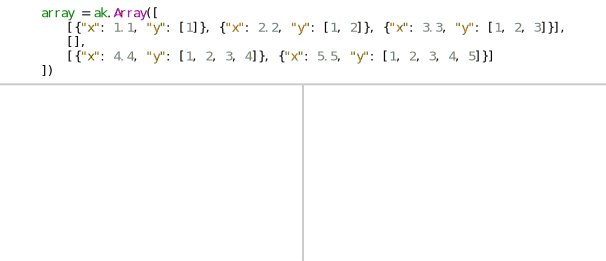
\includegraphics[width=\linewidth]{pivarski-one-slide-summary-1.pdf}}\only<3>{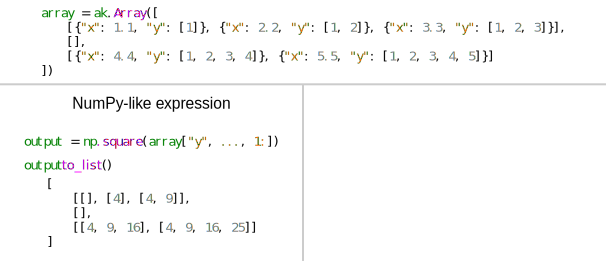
\includegraphics[width=\linewidth]{pivarski-one-slide-summary-2.pdf}}\only<4>{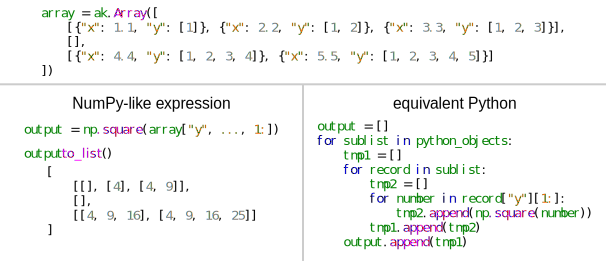
\includegraphics[width=\linewidth]{pivarski-one-slide-summary-3.pdf}}
\end{columns}
\end{frame}

\begin{frame}{History of the project}

\begin{columns}
\column{1.15\linewidth}
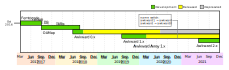
\includegraphics[width=\linewidth]{awkward-timeline.pdf}
\end{columns}

\begin{uncoverenv}<2->
\begin{itemize}
\item Prehistory: Femtocode {\small (\textcolor{darkgreen}{21 kLOC Python})} and OAMap {\small (\textcolor{darkgreen}{8 kLOC Python})}
\item Awkward 0.x: first users, first API, pure Python + NumPy {\small (\textcolor{darkgreen}{9 kLOC Python})}
\item Awkward 1.x: rewrite for stability \& API \mbox{\small (\textcolor{darkgreen}{22 kLOC Python}, \textcolor{blue}{70 kLOC C++}, \textcolor{violet}{14 kLOC C})\hspace{-0.5 cm}}
\item Awkward 2.x: refactor for maintainability \mbox{\small (\textcolor{darkgreen}{29 kLOC Python}, \textcolor{blue}{10 kLOC C++}, \textcolor{violet}{9 kLOC C})\hspace{-0.5 cm}}
\end{itemize}
\end{uncoverenv}
\end{frame}

\begin{frame}{Language changes}
\large
\vspace{0.5 cm}

\textcolor{darkblue}{Awkward 0.x $\to$ 1.x:} complete rewrite with the intention of changing the API.

\vspace{0.25 cm}
Had to replace some NumPy function calls with precompiled C functions, so we also built the infrastructure in C++ with Python only for the high-level front-end.

\vspace{1 cm}
\begin{uncoverenv}<2->
\textcolor{darkblue}{Awkward 1.x $\to$ 2.x:} porting the C++ infrastructure to Python.

\vspace{0.25 cm}
For reasons described later in this talk.

\vspace{0.25 cm}
\begin{center}
\begin{tabular}{c r r}
\textcolor{darkgreen}{Python} & \textcolor{darkgreen}{$-19.6$~kLOC} & \textcolor{darkgreen}{$+26.9$~kLOC} \\
\textcolor{blue}{C++} & \textcolor{blue}{$-59.8$~kLOC} & \textcolor{blue}{$+0$~kLOC} \\
\textcolor{violet}{C} & \textcolor{violet}{$-4.9$~kLOC} & \textcolor{violet}{$+0$~kLOC} \\
\end{tabular}

\vspace{0.25 cm}
\textcolor{gray}{\scriptsize kLOC = thousands of non-blank, non-comment lines of code counted by \mintinline{bash}{cloc}}

\textcolor{gray}{\scriptsize Awkward 2.x is 75\% done; the above is a projection}
\end{center}
\end{uncoverenv}
\end{frame}

\begin{frame}{Evolution of architecture: Awkward \only<1>{0.x}\only<2>{1.x}\only<3>{2.x}}
\vspace{0.25 cm}
\begin{columns}
\column{1.15\linewidth}
\mbox{\hspace{1 cm}\only<1>{\includegraphics[width=\linewidth]{awkward-0-layers.pdf}}\only<2>{\includegraphics[width=\linewidth]{awkward-1-layers.pdf}}\only<3>{\includegraphics[width=\linewidth]{awkward-2-layers.pdf}}}
\end{columns}
\end{frame}

\begin{frame}{Language choice is unrelated to performance}
\large

\vspace{0.25 cm}
All $\mathcal{O}(n)$ operations for arrays of length $n$ are performed in the kernels layer (C).

\vspace{0.15 cm}
Porting the tree structures from C++ to Python has no $\mathcal{O}(n)$ impact.

\vspace{0.15 cm}
\begin{uncoverenv}<2->
\mbox{ } \hfill \textcolor{darkblue}{For an array of length 30~million:} \hfill \mbox{ }

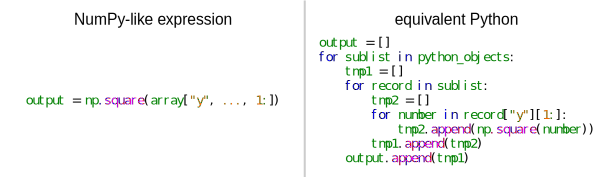
\includegraphics[width=\linewidth]{numpy-like-vs-equivalent-python.pdf}

\vspace{0.25 cm}
\begin{columns}
\column{0.37\linewidth}
Awkward 0.15.5: \hfill\textcolor{darkblue}{4.6~seconds}

Awkward 1.5.1: \hfill\textcolor{darkblue}{2.4~seconds}

Awkward 2.0.0a: \hfill\textcolor{darkblue}{1.5~seconds}

\column{0.4\linewidth}
equivalent Python: \textcolor{darkblue}{140~seconds}

\textcolor{gray}{because $\mathcal{O}(n)$ operations are performed in Python}
\end{columns}
\end{uncoverenv}
\end{frame}


\end{document}

%% Description
%% Awkward Array 0.x was written entirely in Python, and Awkward Array 1.x was a fresh rewrite with a C++ core and a Python interface. Ironically, the Awkward Array 2.x project is translating most of that core back into Python (leaving the interface untouched). This is because we discovered surprising and subtle issues in Python-C++ integration that can be avoided with a more minimal coupling: we can still put performance-critical code in C++, but also benefit by minimizing the interface between the two languages.

%% This talk is intended to share what we learned from our experiences: design choices that look innocent but can cause issues several steps later, often only in the context of real applications. The points to be presented are (1) memory management: although Python references can be glued to std::shared_ptr, cycles through C++ are invisible to Python's garbage collector and can arise in subtle ways, (2) C++ standard library types are not a portable runtime interface, owing to ABI differences, and (3) tracers, at the heart of Python libraries like Dask and JAX, can only be fully leveraged if black-box calls out of Python use basic, universally recognized types: flat arrays, not objects.

%% The goal of this talk is to call out these issues so that other projects mixing Python and C++ can avoid them in the design stage.

%% References
%% The closest match to this talk's content can be found in an IRIS-HEP Analysis Systems group meeting: https://indico.cern.ch/event/1032972/

%% But this talk would be for a wider audience, presenting these issues in a more general way: more like "how to" tips than specific project plans.

%% Significance
%% This talk is not aimed at potential users of Awkward Array, but developers working on other projects that need to mix Python and C++. This need is increasingly relevant as more front-ends use Python, but large-scale processing still needs to have high performance.
